\documentclass[tikz,border=10pt]{standalone}
\usepackage{tikz}
\usetikzlibrary{shapes.geometric,arrows.meta,positioning,calc,backgrounds,shadows,decorations.pathmorphing,fit}
\usepackage[T1]{fontenc}
\usepackage{amssymb}
\usepackage{helvet}\renewcommand{\familydefault}{\sfdefault}
\usepackage[tracking=true]{microtype}

\definecolor{bandA}{HTML}{BBD4F5}
\definecolor{bandB}{HTML}{CDBCEC}
\definecolor{bandC}{HTML}{B9E3C6}
\definecolor{secA}{HTML}{3E6FB4}
\definecolor{secB}{HTML}{6E51A8}
\definecolor{secC}{HTML}{3F8A5E}
\definecolor{cardEdge}{HTML}{51607A}
\definecolor{boxblue}{HTML}{BFD8F7}
\definecolor{boxpurple}{HTML}{D6C8F0}
\definecolor{boxgreen}{HTML}{BFE5CC}
\definecolor{chipadv}{HTML}{F6C7C4}
\definecolor{chipnat}{HTML}{FADFB8}
\definecolor{chipben}{HTML}{CBE9BC}
\definecolor{dbcol}{HTML}{F3E1A8}
\definecolor{dbtop}{HTML}{EAD285}
\definecolor{ink}{HTML}{273244}
\definecolor{sub}{HTML}{5B6779}
\definecolor{arrowc}{HTML}{7A8698}
\definecolor{hi}{RGB}{212,241,212}
\definecolor{lo}{RGB}{250,214,214}
\definecolor{trajgood}{HTML}{22C55E}
\definecolor{trajbad}{HTML}{FF3B30}


\tikzset{
  every node/.style={font=\small, text=ink},
  card/.style={draw=cardEdge!45, rounded corners=2.4mm, fill=white,
               inner sep=2.6mm, line width=0.6pt,
               drop shadow={opacity=0.12, shadow xshift=0.35mm, shadow yshift=-0.55mm,
                            fill=black}},
  model/.style={card, fill=boxblue, minimum width=17mm, minimum height=10mm,
                font=\small\bfseries},
  modelp/.style={model, fill=boxpurple},
  modelg/.style={model, fill=boxgreen},
  chip/.style={draw=cardEdge!35, rounded corners=1.7mm, inner xsep=2.2mm,
               inner ysep=1.5mm, font=\footnotesize, line width=0.5pt,
               drop shadow={opacity=0.10, shadow xshift=0.3mm, shadow yshift=-0.45mm,
                            fill=black}},
  db/.style={cylinder, shape border rotate=90, draw=cardEdge!50, fill=dbcol,
             cylinder uses custom fill, cylinder body fill=dbcol, cylinder end fill=dbtop,
             aspect=0.16, minimum width=14.5mm, minimum height=12.5mm,
             inner sep=1.1mm, line width=0.6pt, font=\footnotesize\bfseries,
             drop shadow={opacity=0.12, shadow xshift=0.35mm, shadow yshift=-0.55mm,
                          fill=black}},
  arr/.style={-{Stealth[length=2.7mm, width=2.2mm]}, line width=0.8pt,
              draw=arrowc, rounded corners=2mm},
  lab/.style={font=\footnotesize, text=sub, inner sep=1pt},
}

\begin{document}
\begin{tikzpicture}

% ================= EVIDENCE GATHERING (top band) =================
\node[card, align=left, inner sep=1.8mm] (task) at (0,0) {%
  \begin{tabular}{@{}l@{}}
  \multicolumn{1}{c}{\footnotesize\bfseries task}\\[0.5mm]
  {\tiny\bfseries scene:}\\[0.2mm]
  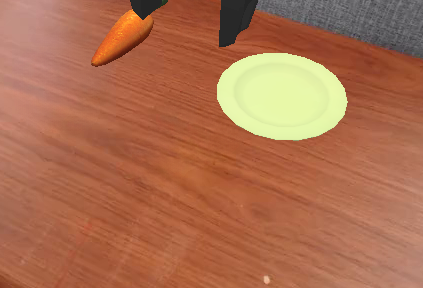
\includegraphics[width=27mm]{frames/method_frame.png}\\[0.5mm]
  {\tiny\bfseries instruction:}\\[0.1mm]
  {\scriptsize``move the carrot to the plate''}
  \end{tabular}};

\node[model] (vlm1) at (3.6,0) {VLM};
\draw[arr] (task) -- (vlm1);

% two rephrase cards with rollout overlays
\node[inner sep=0pt] (imgmcA) at (7.0,1.32) {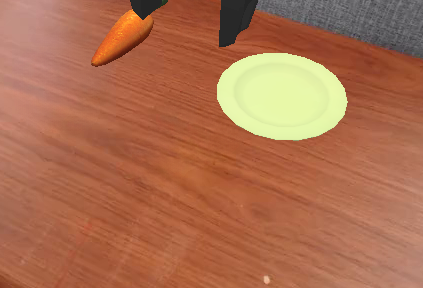
\includegraphics[width=27mm]{frames/method_frame.png}};
\node[lab, anchor=north west, font=\tiny, text=ink] (capmcA) at ($(imgmcA.south west)+(0,-0.06)$) {{\bfseries instruction:} ``move the carrot to the dish''};
\begin{scope}[on background layer]
\node[card, fit=(imgmcA) (capmcA), inner sep=1.4mm] (mcA) {};
\end{scope}
\node[inner sep=0pt] (imgmcB) at (7.0,-1.32) {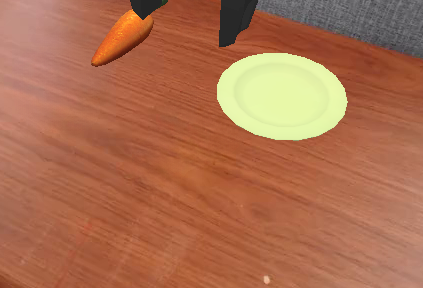
\includegraphics[width=27mm]{frames/method_frame.png}};
\node[lab, anchor=north west, font=\tiny, text=ink] (capmcB) at ($(imgmcB.south west)+(0,-0.06)$) {{\bfseries instruction:} ``place the carrot on the yellow plate''};
\begin{scope}[on background layer]
\node[card, fit=(imgmcB) (capmcB), inner sep=1.4mm] (mcB) {};
\end{scope}

\begin{scope}[trj/.style={line width=0.95pt, line cap=round, dashed, dash pattern=on 1.5pt off 1.0pt,
                          -{Stealth[length=1.6mm, width=1.4mm]}}]
\begin{scope}[shift={(imgmcA.center)}]
\draw[trj, trajgood] (-0.27,0.20) .. controls (-0.15,-0.10) and (0.10,-0.40) .. (0.42,-0.36);
\node[font=\scriptsize\bfseries, text=trajgood] at (0.58,-0.40) {$\checkmark$};
\draw[trj, trajbad]  (-0.27,0.20) .. controls (0.10,0.45) and (0.60,0.55) .. (0.95,0.50);
\node[font=\scriptsize\bfseries, text=trajbad] at (1.08,0.52) {$\times$};
\draw[trj, trajbad]  (-0.27,0.20) .. controls (0.20,0.25) and (0.70,0.12) .. (1.00,0.02);
\node[font=\scriptsize\bfseries, text=trajbad] at (1.13,0.00) {$\times$};
\draw[trj, trajbad]  (-0.27,0.20) .. controls (-0.60,0.05) and (-0.85,-0.30) .. (-0.95,-0.62);
\node[font=\scriptsize\bfseries, text=trajbad] at (-1.05,-0.72) {$\times$};
\end{scope}
\begin{scope}[shift={(imgmcB.center)}]
\draw[trj, trajgood] (-0.27,0.20) .. controls (-0.15,-0.10) and (0.10,-0.40) .. (0.42,-0.36);
\draw[trj, trajgood] (-0.27,0.20) .. controls (0.00,0.00) and (0.25,-0.25) .. (0.50,-0.26);
\draw[trj, trajgood] (-0.27,0.20) .. controls (-0.30,-0.20) and (0.00,-0.55) .. (0.38,-0.48);
\node[font=\scriptsize\bfseries, text=trajgood] at (0.64,-0.36) {$\checkmark$};
\draw[trj, trajbad]  (-0.27,0.20) .. controls (0.20,0.25) and (0.70,0.12) .. (1.00,0.02);
\node[font=\scriptsize\bfseries, text=trajbad] at (1.13,0.00) {$\times$};
\end{scope}
\end{scope}

\coordinate (fork) at (4.85,0);
\draw[line width=0.8pt, draw=arrowc] (vlm1.east) -- node[lab, above=0.8mm, align=center, pos=0.5]{rephrase\\[-0.2mm]\& score} (fork);
\draw[arr] (fork) |- (mcA.west);
\draw[arr] (fork) |- (mcB.west);

% evidence panel
\node[card, align=center, inner sep=1.6mm] (evidence) at (11.1,0) {%
  \begin{tabular}{@{}c@{\hspace{1.2mm}}c@{\hspace{1.2mm}}c@{}}
  \multicolumn{3}{c}{\footnotesize\bfseries evidence}\\[0.9mm]
  \colorbox{lo}{\strut\tiny\bfseries move} & {\tiny vs} & \colorbox{hi}{\strut\tiny\bfseries put}\\[-0.3mm]
  {\tiny the carrot\ldots} & & {\tiny the carrot\ldots}\\[-0.3mm]
  {\tiny\bfseries 25\%} & & {\tiny\bfseries 50\%}\\[1.3mm]
  {\tiny\ldots on the} & & {\tiny\ldots on the}\\[-0.3mm]
  \colorbox{lo}{\strut\tiny\bfseries plate} & {\tiny vs} & \colorbox{hi}{\strut\tiny\bfseries yellow plate}\\[-0.3mm]
  {\tiny\bfseries 15\%} & & {\tiny\bfseries 30\%}\\[1.3mm]
  \colorbox{lo}{\strut\tiny\bfseries \ldots dish} & {\tiny vs} & \colorbox{hi}{\strut\tiny\bfseries \ldots plate}\\[-0.3mm]
  {\tiny\bfseries 10\%} & & {\tiny\bfseries 60\%}
  \end{tabular}};
\draw[arr] (mcA.east) -- ($(evidence.west)+(-0.02,0.9)$);
\draw[arr] (mcB.east) -- ($(evidence.west)+(-0.02,-0.9)$);

% ================= RULE DISTILLATION (right rail) =================
\node[modelp] (llm) at (14.4,0.6) {LLM};
\draw[arr] (evidence.east) -- (evidence.east -| 13.35,0) |- (llm.west);
\node[card, align=left, inner sep=1.8mm] (rules) at (14.4,-2.6) {%
  \begin{tabular}{@{}l@{}}
  \multicolumn{1}{c}{\footnotesize\bfseries rules}\\[0.6mm]
  {\tiny prefer `put' over `move',}\\[-0.2mm]
  {\tiny `place', etc.}\\[0.6mm]
  {\tiny prefer common nouns:}\\[-0.2mm]
  {\tiny keep `plate', not `dish'}\\[0.3mm]
  {\tiny\ldots}
  \end{tabular}};
\draw[arr] (llm) -- node[lab, right=1.2mm]{distill} (rules);

% ================= RULE APPLICATION (bottom band) =================
\node[card, align=left, inner sep=1.6mm] (task2) at (7.0,-5.05) {%
  \begin{tabular}{@{}l@{}}
  \multicolumn{1}{c}{\footnotesize\bfseries task}\\[0.4mm]
  {\tiny\bfseries scene:}\\[0.2mm]
  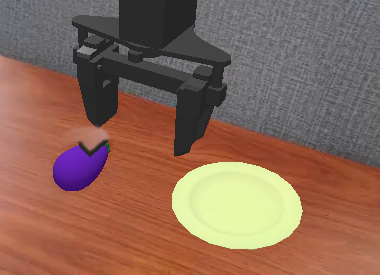
\includegraphics[width=24mm]{frames/eggplant_plate_cropped.png}\\[0.4mm]
  {\tiny\bfseries instruction:}\\[0.1mm]
  {\scriptsize``Can you move the eggplant to the dish?''}
  \end{tabular}};

\node[modelg] (vlm2) at (7.0,-7.45) {VLM};
\node[card, align=center, inner sep=1.6mm] (reph) at (2.9,-7.45) {%
  {\footnotesize\bfseries rephrased task instruction}\\[0.4mm]
  {\scriptsize``put the eggplant on the plate''}};
\node[model] (vla2) at (-0.6,-7.45) {VLA};
\draw[arr] (task2) -- (vlm2);
\draw[arr] (rules.south) |- (vlm2.east);
\draw[arr] (vlm2) -- node[lab, above=0.7mm]{rephrase} (reph);
\draw[arr] (reph) -- (vla2);

% ================= bands =================
\begin{scope}[on background layer]
  \fill[bandA, fill opacity=0.38, rounded corners=4mm]
      (-1.95,2.55) rectangle (12.65,-2.85);
  \fill[bandB, fill opacity=0.38, rounded corners=4mm]
      (12.85,2.55) rectangle (16.0,-8.25);
  \fill[bandC, fill opacity=0.38, rounded corners=4mm]
      (-1.95,-3.05) rectangle (12.65,-8.25);
\end{scope}

% ================= section labels =================
\node[anchor=north west, font=\normalsize\bfseries, text=secA]
  at (-1.85,2.5) {\textls[130]{EVIDENCE GATHERING}};
\node[anchor=north west, font=\normalsize\bfseries, text=secB]
  at (12.95,2.5) {\textls[110]{RULE}};
\node[anchor=north west, font=\normalsize\bfseries, text=secB]
  at (12.95,2.05) {\textls[110]{DISTILLATION}};
\node[anchor=north west, font=\normalsize\bfseries, text=secC]
  at (-1.85,-3.1) {\textls[130]{RULE APPLICATION}};

\end{tikzpicture}
\end{document}
